\documentclass{beamer}
\usepackage{beamerthemesplit}
\usepackage{booktabs}
\RequirePackage{graphicx}
\RequirePackage[italian]{babel}
\usepackage[utf8x]{inputenc}
\usepackage{tikz}
\usetikzlibrary{arrows,shapes}
\tikzstyle{actor edge} = [red!90]
\tikzstyle{director edge} = [blue!90]

\title[LOD CB-RS]{Linked Open Data per un Content-based Recommender System}
\institute{ \textbf{Accesso intelligente alle informazioni ed \\ elaborazione del linguaggio naturale\\}
~ \\
\begin{small}
Corso di Laurea in Informatica Magistrale
\end{small}}
\author{\textbf{Luciano Quercia}\\
\textbf{Simone Rutigliano}}
\date{\tiny{\today}}


%\usetheme{Hannover}
\usetheme{Copenhagen}
\usecolortheme{seahorse}
\usecolortheme{rose}
%\usetheme{Frankfurt}
%\usecolortheme{beetle}

%\useoutertheme[subsection=false]{smoothbars}
%\useoutertheme[subsection=false]{smoothtree}
\useoutertheme{shadow}
\setbeamercovered{dynamic}

\pgfdeclareimage[height=1cm]{logo}{figure/logo}
\logo{\pgfuseimage{logo}}

\begin{document}

%%%%%%%%%%%%%%%%%%%%%%%%%%%%%%%%%%%%%%%%%%%%%%%%%%%%%

\begin{frame}
\maketitle
\end{frame}

%%%%%%%%%%%%%%%%%%%%%%%%%%%%%%%%%%%%%%%%%%%%%%%%%%%%%

\begin{frame}
\frametitle{Outline}
\tableofcontents
\end{frame}

%%%%%%%%%%%%%%%%%%%%%%%%%%%%%%%%%%%%%%%%%%%%%%%%%%%%%

\section{Obiettivi}
\begin{frame}
\frametitle{Obiettivi}
Realizzazione di un \textbf{content-based recommender system}

basato sulla \textbf{Linked Open Data Cloud}
\end{frame}

%%%%%%%%%%%%%%%%%%%%%%%%%%%%%%%%%%%%%%%%%%%%%%%%%%%%%

\begin{frame}
\frametitle{Content-based Recommender System}
Il sistema stabilisce a priori la distanza trai film al fine di raccomandare i più simili alle preferenze dell'utente

\begin{figure}
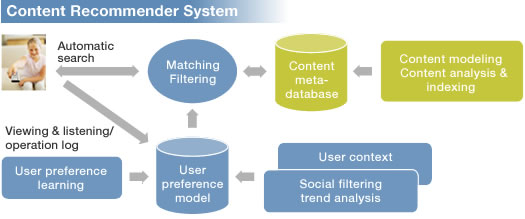
\includegraphics[width=.8\textwidth]{figure/cbrs.jpg}
\end{figure}

\end{frame}

%%%%%%%%%%%%%%%%%%%%%%%%%%%%%%%%%%%%%%%%%%%%%%%%%%%%%

\begin{frame}
\frametitle{Linked Open Data Cloud}

%
\includegraphics[width=.95\textwidth]{figure/LoDLogo.png}

Collezione (\textbf{Cloud}) di dataset:
\begin{itemize}
\item descritti attraverso RDF
\item fortemente interconnessi fra loro (\textbf{Linked})
\item fruibili liberamente e gratuitamente (\textbf{Open})
\end{itemize}
\end{frame}

%%%%%%%%%%%%%%%%%%%%%%%%%%%%%%%%%%%%%%%%%%%%%%%%%%%%%

\begin{frame}
\frametitle{Linked Open Data Cloud}
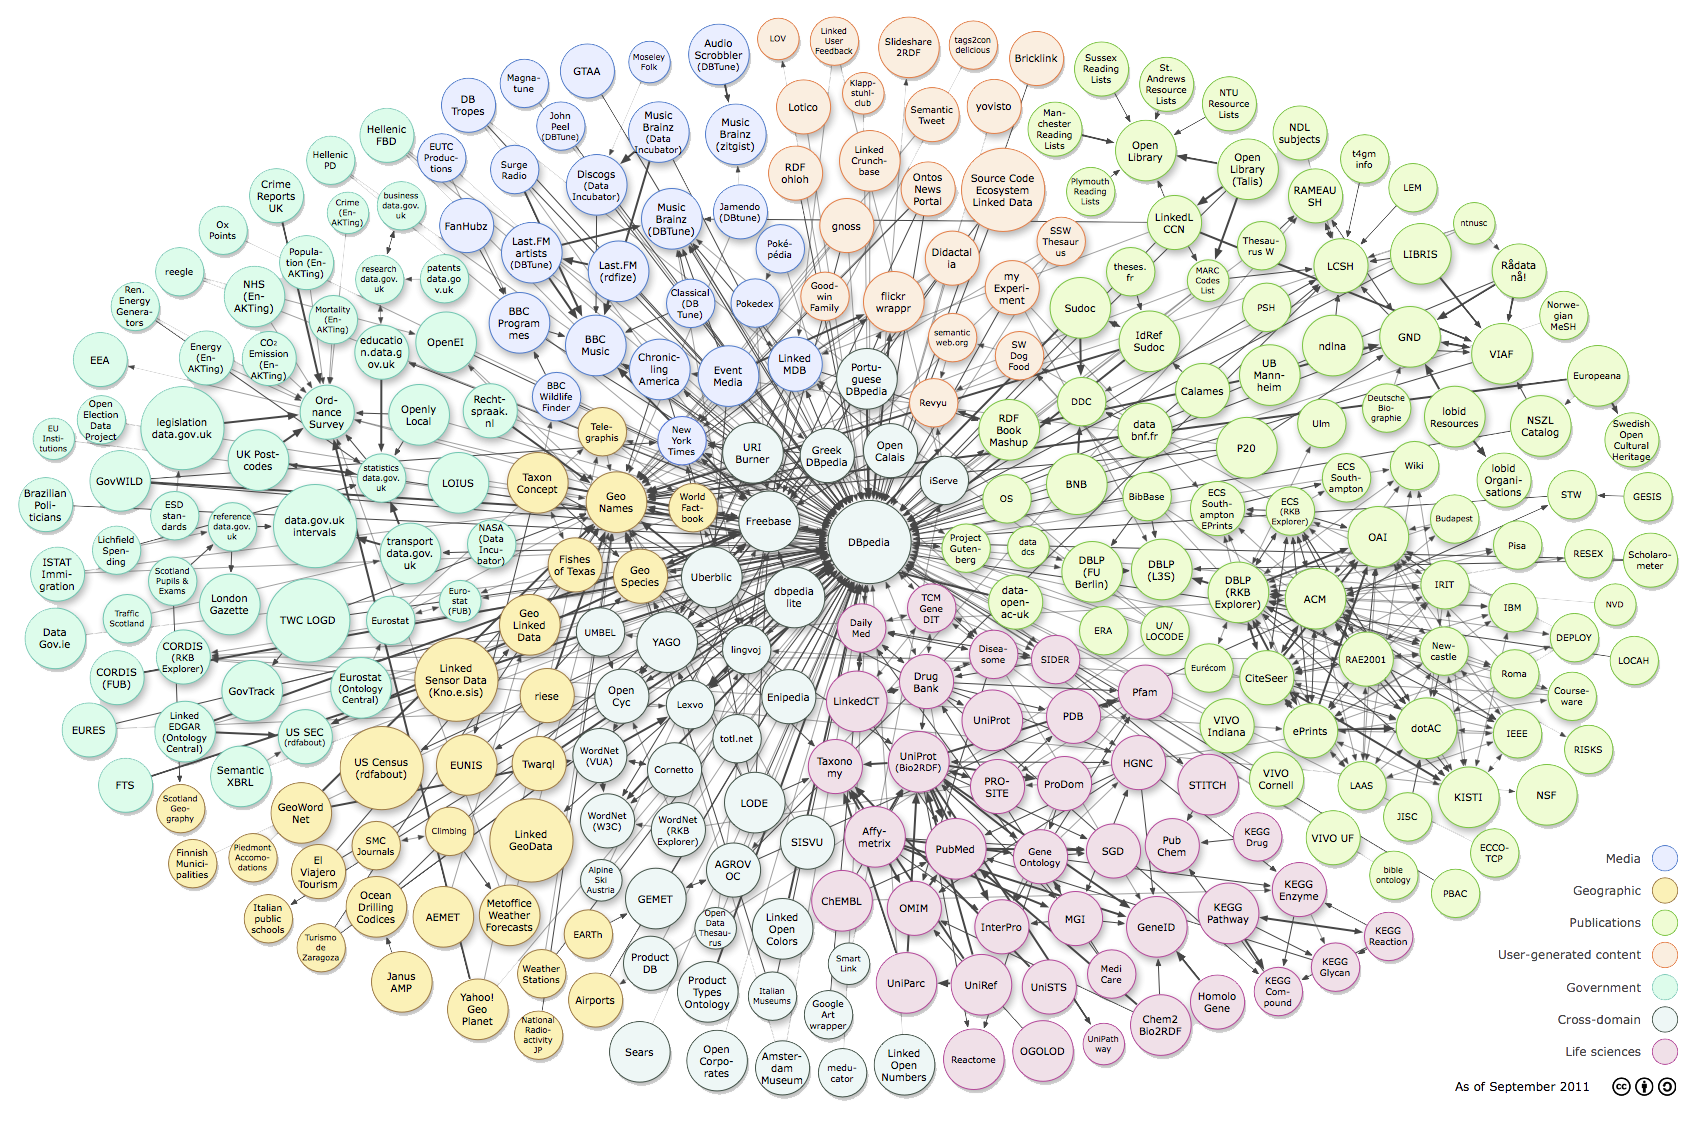
\includegraphics[width=.95\textwidth]{figure/lodcloud}
\end{frame}

%%%%%%%%%%%%%%%%%%%%%%%%%%%%%%%%%%%%%%%%%%%%%%%%%%%%%

\begin{frame}
\frametitle{Resource Description Framework}
Strumento base proposto da \emph{W3C} per la codifica, lo scambio e il riutilizzo di metadati strutturati.

L'RDF Data Model si basa su tre principi chiave:
\begin{enumerate}
\item qualunque cosa può essere identificata da un (URI)
\item utilizzare il linguaggio meno espressivo per definire qualunque cosa
\item qualunque cosa può dire qualunque cosa su qualunque cosa
\end{enumerate}
\end{frame}

%%%%%%%%%%%%%%%%%%%%%%%%%%%%%%%%%%%%%%%%%%%%%%%%%%%%%

\begin{frame}
\frametitle{Esempio - Resource Description Framework}
Considerando la frase:\\~\\
\begin{center} \emph{Tarantino is the director of the Django Unchained.} \\~\\
\end{center}
L'affermazione può essere suddivisa come: \\~\\
\begin{tabular}{ l | l }
    Soggetto (Risorsa) & Django Unchained \\
    Predicato (Proprietà) & director \\
    Oggetto (letterale) & Tarantino \\
\end{tabular}
\end{frame}

%%%%%%%%%%%%%%%%%%%%%%%%%%%%%%%%%%%%%%%%%%%%%%%%%%%%%

\section{Progetto}

\subsection{Sorgente dati}

\begin{frame}
\frametitle{DBPedia}
\begin{itemize}
\item Centro della Linked Open Data Cloud
\item Dump di Wikipedia trasformato in RDF
\end{itemize}
\begin{figure}

\includegraphics[width=.30\textwidth]{figure/dbpedia_logo}
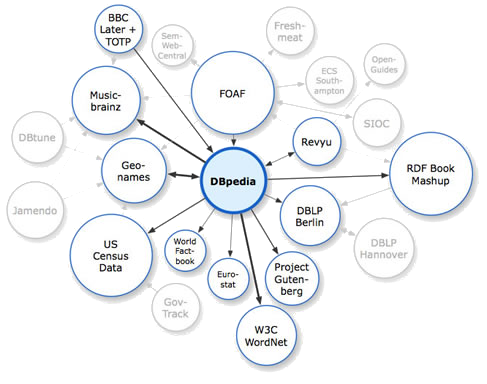
\includegraphics[width=.60\textwidth]{figure/AboutDBPedia}
\end{figure}
\end{frame}

\begin{frame}
\frametitle{Proprietà estratte}
Per la raccomandazione di film, abbiamo estratto le seguenti proprietà
\begin{columns}
\column[t]{5cm}
\begin{itemize}
\item studio
\item music
\item music composer
\item writer
\item editing
\item director
\end{itemize}
\column[t]{5cm}
\begin{itemize}
\item subject
\item starring
\item productor
\item writer
\item cinematography
\end{itemize}
\end{columns}
\end{frame}

%%%%%%%%%%%%%%%%%%%%%%%%%%%%%%%%%%%%%%%%%%%%%%%%%%%%%

\subsection{Realizzazione}

%%%%%%%%%%%%%%%%%%%%%%%%%%%%%%%%%%%%%%%%%%%%%%%%%%%%%

\begin{frame}
\frametitle{Grafo delle Risorse}
Attraverso query SPARQL sono state estratte tutte le triple che avevano proprietà nota e un film come soggetto
è stato generato il grafo delle risorse

%\begin{verbatim}
%PREFIX dbpedia: <http://dbpedia.org/resource/>
%PREFIX prop: <http://dbpedia.org/ontology/>
%SELECT ?name
%WHERE {
%  dbpedia:Django\_Unchained prop:director ?name .
%}
%\end{verbatim}

\begin{tabular}{|c|}
  \hline
  name \\
  \hline
  http://dbpedia.org/resource/Quentin\_Tarantino \\
  \hline
\end{tabular}
\end{frame}

%%%%%%%%%%%%%%%%%%%%%%%%%%%%%%%%%%%%%%%%%%%%%%%%%%%%%

\begin{frame}
\frametitle{Grafo dei Film}
Tutte le risorse non film sono state epurate ed inglobate all'interno degli archi.

\begin{columns}[p]
\begin{column}{0.8\textwidth} 
\begin{tikzpicture}
[lineDecorate/.style={-,thick},%
  actor/.style={shape=circle,inner sep=3pt,draw, thick},
  film/.style={shape=diamond,inner sep=4pt,draw,thick, fill=blue!15}]

%% nodes or vertices
\foreach \nodename/\x/\y/\direction/\navigate in {
  $Django Unchained$/1/3/left/west, $Inglourious Basterds$/3/3/right/east, $Titanic$/1/1/below/south}
{
  \node (\nodename) at (\x,\y) [film] {};
  \node [\direction] at (\nodename.\navigate) {\footnotesize$\nodename$};
}

\foreach \nodename/\x/\y/\direction/\navigate in {
  $Quentin Tarantino$/2/4/above/north, $Leonardo Di caprio$/1/2/left/west, $Christoph Waltz$/3/2/right/east}
{
  \node (\nodename) at (\x,\y) [actor] {};
  \node [\direction] at (\nodename.\navigate) {\footnotesize$\nodename$};
}

%% edges or lines
\path
\foreach \startnode/\endnode in {$Django Unchained$/$Leonardo Di caprio$, $Django Unchained$/$Christoph Waltz$, $Inglourious Basterds$/$Christoph Waltz$, $Leonardo Di caprio$/$Titanic$}
{
  (\startnode) edge[lineDecorate,director edge] node {} (\endnode)
}

\foreach \startnode/\endnode in {$Django Unchained$/$Quentin Tarantino$,$Quentin Tarantino$/$Inglourious Basterds$}
{
  (\startnode) edge[lineDecorate,bend left,actor edge] node {} (\endnode)
}

\foreach \startnode/\endnode in {$Quentin Tarantino$/$Django Unchained$, $Inglourious Basterds$/$Quentin Tarantino$}
{
  (\startnode) edge[lineDecorate,bend left,director edge] node {} (\endnode)
};

\end{tikzpicture}
\end{column}

\begin{column}{0.2\textwidth}
\begin{tabbing}
  Simbolo \= Valore \kill
  % \> for next tab, \\ for new line...
  a \> Film \\
  b \> Actor \\
  c \> Edge director \\
  d \> Edge actor
\end{tabbing}
\end{column}
\end{columns}
\end{frame}

%%%%%%%%%%%%%%%%%%%%%%%%%%%%%%%%%%%%%%%%%%%%%%%%%%%%%

\subsection{Fattori}

%%%%%%%%%%%%%%%%%%%%%%%%%%%%%%%%%%%%%%%%%%%%%%%%%%%%%

\begin{frame}
\frametitle{Distanze}
Sono state applicate 4 distanze su grafo:

\begin{itemize}
\item Direct
\item Combinated
\item Direct Weighted
\item Combinated Weighted
\end{itemize}
\end{frame}

%%%%%%%%%%%%%%%%%%%%%%%%%%%%%%%%%%%%%%%%%%%%%%%%%%%%%

\begin{frame}
\frametitle{Rappresentazione del profilo}
Il profilo è stato rappresentato in 2 modi:

\begin{itemize}
\item[Simple] Insieme di film positivi per l'utente
\item[Weighted] Ogni film influisce, positivamente o negativamente, alle raccomandazioni, secondo il voto ricevuto
\end{itemize}


\end{frame}

%%%%%%%%%%%%%%%%%%%%%%%%%%%%%%%%%%%%%%%%%%%%%%%%%%%%%

\subsection{Output}

%%%%%%%%%%%%%%%%%%%%%%%%%%%%%%%%%%%%%%%%%%%%%%%%%%%%%

\begin{frame}
\frametitle{Raccomandazioni}
\end{frame}

%%%%%%%%%%%%%%%%%%%%%%%%%%%%%%%%%%%%%%%%%%%%%%%%%%%%%

\section{Sperimentazione}
\subsection{Dataset}

%%%%%%%%%%%%%%%%%%%%%%%%%%%%%%%%%%%%%%%%%%%%%%%%%%%%%

\begin{frame}
\frametitle{MovieLens}
\end{frame}

%%%%%%%%%%%%%%%%%%%%%%%%%%%%%%%%%%%%%%%%%%%%%%%%%%%%%

\subsection{Protocollo Sperimentale}

%%%%%%%%%%%%%%%%%%%%%%%%%%%%%%%%%%%%%%%%%%%%%%%%%%%%%

\begin{frame}
\frametitle{Protocollo Sperimentale}
\end{frame}

%%%%%%%%%%%%%%%%%%%%%%%%%%%%%%%%%%%%%%%%%%%%%%%%%%%%%

\begin{frame}
\frametitle{Metriche}
\end{frame}

%%%%%%%%%%%%%%%%%%%%%%%%%%%%%%%%%%%%%%%%%%%%%%%%%%%%%

\subsection{Risultati}

%%%%%%%%%%%%%%%%%%%%%%%%%%%%%%%%%%%%%%%%%%%%%%%%%%%%%

\begin{frame}
\frametitle{Risultati}
\end{frame}

%%%%%%%%%%%%%%%%%%%%%%%%%%%%%%%%%%%%%%%%%%%%%%%%%%%%%

\section{Conclusioni e sviluppi futuri}
\begin{frame}
\frametitle{Conclusioni e sviluppi futuri}
\end{frame}

%%%%%%%%%%%%%%%%%%%%%%%%%%%%%%%%%%%%%%%%%%%%%%%%%%%%%

\begin{frame}
\frametitle{TEPaC}
TEPaC

\emph{Transductive Emerging Pattern based Classifier}

\begin{itemize}
\item classificatore di strutture logiche
\item basato su pattern emergenti
\item utilizza un approccio trasduttivo
\end{itemize}

\end{frame}

%%%%%%%%%%%%%%%%%%%%%%%%%%%%%%%%%%%%%%%%%%%
%%%%%%%%%%%%%%%%%%%%%%%%%%%%%%%%%%%%%%%%%%%
%%%%%%%%%%%%%%%%%%%%%%%%%%%%%%%%%%%%%%%%%%%

\subsection{Document Image Understanding}
\begin{frame}
\frametitle{Document Image Understanding}

\begin{columns}
\begin{column}{0.6\textwidth}

\begin{itemize}
\item<1-> Comprensione automatizzata di documenti cartacei
\item<2-> La maggior parte della conoscenza mondiale si trova su supporti cartacei
\begin{itemize}
\item Libri
\item Documenti
\item Giornali
\end{itemize}
\item<3-> La digitalizzazione offre innumerevoli vantaggi
\end{itemize}
\end{column}

\begin{column}{0.2\textwidth}
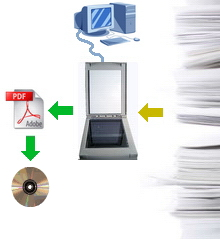
\includegraphics[width=3cm]{figure/diu.jpg}
\end{column}

\end{columns}

\end{frame}


%%%%%%%%%%%%%%%%%%%%%%%%%%%%%%%%%%%%%%%%%%%
%%%%%%%%%%%%%%%%%%%%%%%%%%%%%%%%%%%%%%%%%%%
%%%%%%%%%%%%%%%%%%%%%%%%%%%%%%%%%%%%%%%%%%%


\begin{frame}
\begin{scriptsize}

\begin{columns}
\begin{column}{0.4\textwidth}
	\begin{tabular}{c | ccc}
	\toprule
	 & \multicolumn{3}{c}{$minSup\ (\%)$} \\
	$minGR$ & 30 & 40 & 50 \\
	\hline
	1  & 528032 & 344798 & 254805 \\
	2  & 523274 & 341534 & 252355 \\
	8  & 516958 & 336733 & 248658 \\
	64 & 513503 & 334292 & 246843 \\
	\bottomrule
	\end{tabular}
Dataset TPAMI
	\vspace{8 mm}
	
	\begin{tabular}{c | ccc}
	\toprule
	 & \multicolumn{3}{c}{$minSup\ (\%)$} \\
	$minGR$ & 10 & 20 & 30 \\
	\hline
	1  & 386996 & 176407 & 114492 \\
	2  & 382639 & 173372 & 112476 \\
	8  & 376645 & 169406 & 109814 \\
	64 & 374736 & 167742 & 108595 \\
	\bottomrule
	\end{tabular}
Dataset ICML

\end{column}

\begin{column}{0.4\textwidth}
	\begin{tabular}{c | ccc}
	\toprule
	 & \multicolumn{3}{c}{$minSup\ \ (\%)$} \\
	$minGR$ & 10 & 20 & 30 \\
	\hline
	1  & 128327 & 88684 & 58603 \\
	2  & 126840 & 87644 & 58091 \\
	8  & 122591 & 84208 & 55718 \\
	64 & 121363 & 82980 & 54490 \\
	\bottomrule
	\end{tabular}
Dataset BG

\end{column}
\end{columns}

\end{scriptsize}
\end{frame}


\begin{frame}
\begin{center}
Grazie per l'attenzione.
\end{center}
\end{frame}
\end{document}
